\chapter[Perturbative Methods and Functional Identities]{Perturbative Methods and\\Functional Identities}

With the rigorously gauge-fixed action established via BRST quantization, one is fully equipped to extract the perturbative dynamics and quantum corrections of gauge theories. We begin this chapter by explicitly deriving the momentum-space Feynman rules for perturbative Quantum Chromodynamics (QCD) and performing the fundamental loop calculations that yield the QCD \(\beta\)-function. This analysis famously reveals the phenomenon of asymptotic freedom, demonstrating exactly how the strong coupling constant evolves with the energy scale.

Beyond diagrammatic perturbation theory, the path integral formalism provides a remarkably unified and elegant framework for encoding the complete quantum dynamics of a system into functional objects known as generating functionals. By formally coupling the quantum fields to external sources, one can systematically generate arbitrary time-ordered correlation functions through straightforward functional differentiation. Furthermore, this functional language allows one to cleanly isolate the physically relevant connected and one-particle-irreducible (1PI) diagrams via the quantum effective action. Ultimately, we will use this powerful functional arena, combined with the quantum equations of motion (Schwinger--Dyson equations), to directly translate the continuous symmetries of the classical action into exact, non-perturbative quantum constraints, culminating in the derivation of the generalized Ward--Takahashi identities that govern the underlying symmetries of the quantum theory.

\section{QCD and the $\beta$-function}

Quantum Chromodynamics (QCD) stands as the foundational non-abelian gauge theory of the strong interaction, describing the intricate dynamics of quarks and gluons charged under the \(SU(3)\) color group. Having established the rigorous framework of BRST quantization and the Faddeev-Popov gauge-fixing procedure for generic Yang-Mills theories, we now explicitly specialize our discussion to the physical case of QCD.

In this section, we will systematically extract the momentum-space Feynman rules directly from the complete gauge-fixed action, providing the essential building blocks required for high-energy perturbative calculations. Building upon these rules, we will explore the renormalization of the theory at the one-loop level, highlighting how the residual BRST symmetry (encoded mathematically in the Slavnov-Taylor identities) tightly constrains the various renormalization constants. This perturbative analysis ultimately culminates in the computation of the defining QCD \(\beta\)-function, which famously reveals the profound phenomenon of asymptotic freedom, dictating that the strong coupling becomes vanishingly small at asymptotically high energy scales. Furthermore, we will demonstrate how the underlying BRST symmetry continues to enforce critical physical consistency conditions, such as generalized Ward identities, thereby rigorously guaranteeing the transversality and gauge-independence of physical scattering amplitudes.

\subsection{Feynman Rules for Perturbative QCD}

Having successfully obtained the completely gauge-fixed action for non-abelian gauge theories, whether by employing the Faddeev-Popov method or the more general BRST method, one can definitively identify the \uline{full QCD gauge-fixed Lagrangian} by systematically adding the matter fermions (specifically, the quark fields). Employing an arbitrary covariant $R_\xi$ gauge, one straightforwardly obtains the complete gauge-fixed Lagrangian.

We remind the reader of our chosen conventions for the metric, Clifford algebra, and Lie algebra generators:
\[\eta_{\mu\nu} = \text{diag}(-, +, +, +), \qquad \{\gamma^\mu, \gamma^\nu\} = 2\eta^{\mu\nu}, \qquad [T^a, T^b] = i f^{abc} T^c,\]
together with the explicit definitions of the covariant derivatives acting on the fundamental and adjoint representations:
\[D_\mu\psi^i = \partial_\mu\psi^i - i g A_\mu^a (T^a)^i_{\phantom{i}j} \psi^j, \qquad D_\mu c^a = \partial_\mu c^a + g f^{abc} A_\mu^b c^c.\]
In what follows, to avoid notational clutter, the specific color index $i$, strictly associated with the fermion representation, is left entirely implicit.

With these established conventions, the complete gauge-fixed Lagrangian evaluated in an arbitrary $R_\xi$ gauge explicitly reads:
\begin{equation} \label{eq:qcd_lagrangian_full}
    \mathcal{L}_{tot} = -\frac{1}{4}F_{\mu\nu}^a F^{a\mu\nu} - B^a\partial^\mu A_\mu^a + \frac{\xi}{2}(B^a)^2 - \partial^\mu \bar{c}^a D_\mu c^a - \sum_{f=1}^6 \overline{\psi}_f(\gamma^\mu D_\mu + m_f)\psi_f
\end{equation}
which can be elegantly rewritten, after systematically eliminating the non-dynamical auxiliary field $B^a$ by substituting its own algebraic equations of motion ($B^a = \frac{1}{\xi}\partial^\mu A_\mu^a$), as:
\begin{equation} \label{eq:qcd_lagrangian_fixed}
    \boxed{\mathcal{L}_{tot} = -\frac{1}{4}F_{\mu\nu}^a F^{a\mu\nu} - \frac{1}{2\xi}(\partial^\mu A_\mu^a)^2 - \partial^\mu \bar{c}^a D_\mu c^a - \sum_{f=1}^6 \overline{\psi}_f(\gamma^\mu D_\mu + m_f)\psi_f \, .}
\end{equation}
This fundamental expression serves as the rigorous starting point for mathematically implementing perturbation theory: the total Lagrangian is systematically split as $\mathcal{L}_{tot} = \mathcal{L}_2 + \mathcal{L}_{int}$, where the strictly quadratic part $\mathcal{L}_2$ unequivocally fixes the free propagators, and the interacting part $\mathcal{L}_{int}$ provides the diverse elementary interaction vertices.

Recalling the explicit expansion of the non-abelian field strength tensor
\begin{equation} \label{eq:field_strength_expansion}
    F_{\mu\nu}^a = \partial_\mu A_\nu^a - \partial_\nu A_\mu^a + g f^{abc} A_\mu^b A_\nu^c \, ,
\end{equation}
one explicitly finds, up to total spacetime derivatives that do not affect the action,
\begin{equation} \label{eq:qcd_lagrangian_quadratic}
    \mathcal{L}_2 = -\frac{1}{2}(\partial_\mu A_\nu^a)^2 + \left(\frac{1}{2} - \frac{1}{2\xi}\right)(\partial^\mu A_\mu^a)^2 - \partial^\mu \bar{c}^a \partial_\mu c^a - \sum_{f=1}^6 \overline{\psi}_f(\gamma^\mu \partial_\mu + m_f)\psi_f \, ,
\end{equation}
and the corresponding interaction terms are grouped as:
\begin{equation} \label{eq:qcd_lagrangian_interaction}
    \mathcal{L}_{int} = - g f^{abc} \partial^\mu A^{\nu a} A_\mu^b A_\nu^c - \frac{g^2}{4} f^{abc} f^{ade} A_\mu^b A_\nu^c A^{\mu d} A^{\nu e} - g f^{abc} \partial^\mu \bar{c}^a A_\mu^b c^c + i g A_\mu^a \sum_{f=1}^6 \overline{\psi}_f \gamma^\mu T^a \psi_f \, .
\end{equation}
It is a profound consequence of the underlying gauge symmetry that all interaction vertices are universally controlled by the exact same fundamental coupling constant $g$.

\subsubsection{Propagators}

The perturbative momentum-space propagators are mathematically defined as the precise inverses of the ``kinetic'' terms, i.e., the specific differential operators contained strictly within the quadratic Lagrangian $\mathcal{L}_2$. In a generalized hypercondensed notation (applicable for generic real fields $\phi^i$ and complex fields $\psi^i, \overline{\psi}_i$, whether they are commuting or anticommuting in nature), one formally has the inversion relations:
\begin{equation} \label{eq:propagator_inversion}
    \begin{aligned}
        S[\phi]                  & = -\frac{1}{2}\phi^i K_{ij} \phi^j             & \quad \rightarrow \quad & \langle \phi^i \phi^j \rangle = -i G^{ij}                        & \quad & (K_{ij}G^{jk} = \delta_i^k)  \, ,                        \\
        S[\psi, \overline{\psi}] & = -\overline{\psi}_i K^i_{\phantom{i}j} \psi^j & \quad \rightarrow \quad & \langle \psi^i \overline{\psi}_j \rangle = -i G^i_{\phantom{i}j} & \quad & (K^i_{\phantom{i}j}G^j_{\phantom{j}k} = \delta^i_k) \, .
    \end{aligned}
\end{equation}

Thus, by systematically inverting the kinetic operators extracted from $\mathcal{L}_2$, we rigorously obtain the required momentum-space propagators:
\begin{equation} \label{eq:qcd_propagators}
    \begin{aligned}
        \langle A_\mu^a(x) A_\nu^b(y) \rangle          & = -i \int \frac{d^4p}{(2\pi)^4} \, e^{ip(x-y)} \, \frac{\delta^{ab}}{p^2 - i\epsilon} \left( \eta_{\mu\nu} - (1 - \xi)\frac{p_\mu p_\nu}{p^2} \right) \, , \\
        \langle c^a(x) \bar{c}^b(y) \rangle            & = -i \int \frac{d^4p}{(2\pi)^4} \, e^{ip(x-y)} \, \frac{\delta^{ab}}{p^2 - i\epsilon} \, ,                                                                 \\
        \langle \psi_f(x) \overline{\psi}_f(y) \rangle & = -i \int \frac{d^4p}{(2\pi)^4} \, e^{ip(x-y)} \, \frac{-i\not{p} + m_f}{p^2 + m_f^2 - i\epsilon} \, ,
    \end{aligned}
\end{equation}
with absolutely no sum over the index $f$ (which strictly denotes the distinct quark flavours). In pure momentum space, the corresponding graphical Feynman rules are thus definitively given by:

\begin{figure}[H]
    \centering
    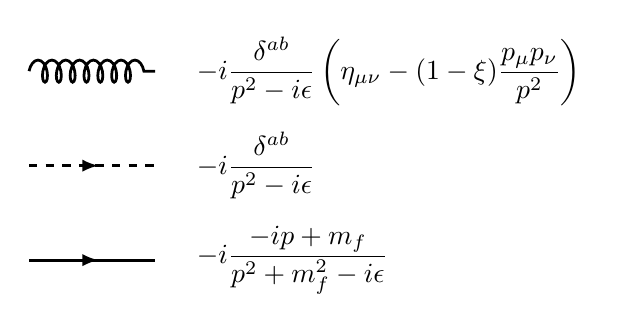
\begin{tikzpicture}[scale=0.8, thick, font=\sffamily]

        % Gluon propagator
        \draw[line width=1pt, decorate, decoration={coil, amplitude=4pt, segment length=5pt}] (-2, 1.5) -- (0, 1.5);
        \node[right] at (0.5, 1.5) {$\displaystyle -i \frac{\delta^{ab}}{p^2 - i\epsilon} \left( \eta_{\mu\nu} - (1 - \xi)\frac{p_\mu p_\nu}{p^2} \right)$};

        % Ghost propagator
        \draw[line width=1pt, dashed] (-2, 0) -- (0, 0);
        \draw[line width=1pt, -latex] (-1.1, 0) -- (-0.9, 0); % arrow
        \node[right] at (0.5, 0) {$\displaystyle -i \frac{\delta^{ab}}{p^2 - i\epsilon}$};

        % Fermion propagator
        \draw[line width=1pt] (-2, -1.5) -- (0, -1.5);
        \draw[line width=1pt, -latex] (-1.1, -1.5) -- (-0.9, -1.5); % arrow
        \node[right] at (0.5, -1.5) {$\displaystyle -i \frac{-i\slashed{p} + m_f}{p^2 + m_f^2 - i\epsilon}$};

    \end{tikzpicture}
\end{figure}

\subsubsection{Vertices}

\uline{The interaction vertices evaluated in momentum space are mathematically obtained by system- atically Fourier transforming the various interaction monomials contained within $\mathcal{L}_{int}$}. Let us therefore briefly revisit our established Fourier transform conventions specifically for the effective action $\Gamma[\varphi] = S_{tot}[\varphi] + \text{loop corrections}$\footnote{This object is conceptually identical to the ``quantum action'' discussed in Srednicki's textbook; see Chapter 21.}, and the intimately related \textit{proper vertices} (which strictly correspond to amputated 1PI Feynman graphs) which are mathematically generated by it. When formally replacing the full quantum effective action $\Gamma[\varphi]$ by the tree-level classical action $S_{tot}[\varphi]$, the full proper vertices are naturally replaced by the bare classical vertices directly entering the fundamental Feynman rules.

The effective action $\Gamma[\varphi]$ evaluated for a generic field $\varphi$ is systematically expanded in a functional Taylor series as:
\begin{equation} \label{eq:effective_action_expansion}
    \begin{aligned}
        \Gamma[\varphi] & = \sum_{n=0}^\infty \frac{1}{n!} \int d^D x_1 \dots d^D x_n \, \Gamma^{(n)}(x_1, \dots, x_n) \, \varphi(x_1) \cdots \varphi(x_n)                                                                                        \\
                        & = \sum_{n=0}^\infty \frac{1}{n!} \int \frac{d^D p_1}{(2\pi)^D} \dots \frac{d^D p_n}{(2\pi)^D} \, \tilde{\Gamma}^{(n)}(p_1, \dots, p_n) \, \tilde{\varphi}(p_1) \cdots \tilde{\varphi}(p_n)                              \\
                        & = \sum_{n=0}^\infty \frac{1}{n!} \int \frac{d^D p_1}{(2\pi)^D} \dots \frac{d^D p_n}{(2\pi)^D} \, (2\pi)^D \delta^D(p_1 + \dots + p_n) \Gamma^{(n)}(p_1, \dots, p_n) \, \tilde{\varphi}(p_1) \cdots \tilde{\varphi}(p_n)
    \end{aligned}
\end{equation}
where the rigorous Fourier transform of the proper vertices with strictly \textit{ingoing momenta} are defined as:
\begin{equation} \label{eq:proper_vertices_ft}
    \begin{aligned}
        \tilde{\Gamma}^{(n)}(p_1, \dots, p_n) & = \int d^D x_1 \dots d^D x_n \, e^{i p_1 x_1 + \dots + i p_n x_n} \, \Gamma^{(n)}(x_1, \dots, x_n) \\
                                              & = (2\pi)^D \delta^D(p_1 + \dots + p_n) \Gamma^{(n)}(p_1, \dots, p_n)
    \end{aligned}
\end{equation}
the second line logically following directly from the fundamental translational invariance of the coordinate-space vertex $\Gamma^{(n)}(x_1, \dots, x_n)$ (which guarantees total momentum conservation), while the standard Fourier transform of the fields with explicitly \textit{outgoing momenta} are defined as:
\begin{equation} \label{eq:field_ft}
    \tilde{\varphi}(p) = \int d^D x \, e^{-ipx} \varphi(x) \, , \qquad \varphi(x) = \int \frac{d^D p}{(2\pi)^D} \, e^{ipx} \tilde{\varphi}(p)
\end{equation}
From this specific convention, we can clearly see that the spacetime derivative maps as $\partial_\mu \rightarrow ip_\mu$ in momentum space, distinctly indicating momentum physically exiting from the field and entering the proper graph $\Gamma^{(n)}(p_1, \dots, p_n)$.

Graphically, these vital correlation functions may be intuitively depicted by:

\begin{figure}[H]
    \centering
    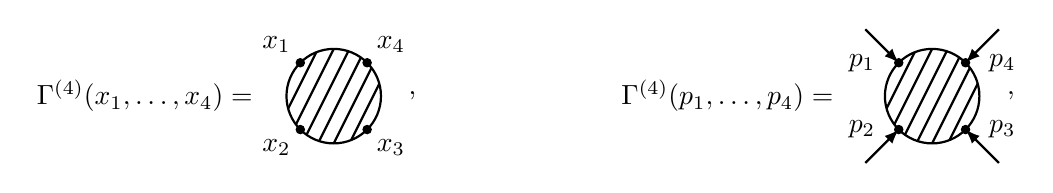
\begin{tikzpicture}[scale=1]

        % First Diagram
        \node at (-2.4, 0) {$\Gamma^{(4)}(x_1, \ldots, x_4) = $};

        \begin{scope}[shift={(0,0)}]
            \draw[thick, fill=white] (0,0) circle (0.6);
            \clip (0,0) circle (0.6);
            \foreach \x in {-1,-0.8,...,1}
            \draw[thick] (\x,-1) -- (\x+1,1);
        \end{scope}

        \filldraw[black] (135:0.6) circle (1.5pt) node[above left] {$x_1$};
        \filldraw[black] (225:0.6) circle (1.5pt) node[below left] {$x_2$};
        \filldraw[black] (315:0.6) circle (1.5pt) node[below right] {$x_3$};
        \filldraw[black] (45:0.6) circle (1.5pt) node[above right] {$x_4$};

        \node at (1, 0) {,};

        % Second Diagram
        \node at (5, 0) {$\Gamma^{(4)}(p_1, \ldots, p_4) = $};

        \begin{scope}[shift={(7.6,0)}]
            \draw[thick, fill=white] (0,0) circle (0.6);
            \clip (0,0) circle (0.6);
            \foreach \x in {-1,-0.8,...,1}
            \draw[thick] (\x,-1) -- (\x+1,1);
        \end{scope}

        \begin{scope}[shift={(7.6,0)}]
            \draw[thick, -latex] (135:1.2) -- (135:0.6);
            \draw[thick, -latex] (225:1.2) -- (225:0.6);
            \draw[thick, -latex] (315:1.2) -- (315:0.6);
            \draw[thick, -latex] (45:1.2) -- (45:0.6);

            \filldraw[black] (135:0.6) circle (1.5pt) node[left=5pt] {$p_1$};
            \filldraw[black] (225:0.6) circle (1.5pt) node[left=5pt] {$p_2$};
            \filldraw[black] (315:0.6) circle (1.5pt) node[right=5pt] {$p_3$};
            \filldraw[black] (45:0.6) circle (1.5pt) node[right=5pt] {$p_4$};
        \end{scope}

        \node at (8.6, 0) {,};


    \end{tikzpicture}
\end{figure}

where in the second graph, overall conservation of momentum is implicitly understood, and the external directed lines strictly indicate the physical flow of momentum but crucially do not include the external propagators themselves (i.e., the 1PI graphs are fully amputated).

In particular, analyzing the expansion, one finds that $\Gamma^{(0)}$ is simply the zero-point function (vacuum bubble), $\Gamma^{(1)}(p)$ is the one-point function (tadpole), which is often systematically set to vanish by appropriately adjusting the Vacuum Expectation Value (VEV) of the quantum field $\varphi(p)$, and crucially, $\Gamma^{(2)}(-p, p)$ represents the full effective kinetic term contained in the expansion:
\begin{equation} \label{eq:effective_kinetic_term}
    \begin{aligned}
        \Gamma^{(2)}(\varphi) & = \frac{1}{2} \int \frac{d^D p_1}{(2\pi)^D} \frac{d^D p_2}{(2\pi)^D} \, (2\pi)^D \delta^D(p_1 + p_2) \Gamma^{(2)}(p_1, p_2) \tilde{\varphi}(p_1) \tilde{\varphi}(p_2) \\
                              & = \frac{1}{2} \int \frac{d^D p}{(2\pi)^D} \, \tilde{\varphi}(-p) \Gamma^{(2)}(-p, p) \tilde{\varphi}(p)                                                               \\
                              & = \frac{1}{2} \int \frac{d^D p}{(2\pi)^D} \, \tilde{\varphi}(-p) \left( -p^2 - m^2 + \Pi(p^2) \right) \tilde{\varphi}(p)
    \end{aligned}
\end{equation}
where $-p^2 - m^2$ is exactly the tree-level classical kinetic term whose mathematical inverse (multiplied by $i$) directly gives the standard perturbative propagator in momentum space $\frac{-i}{p^2 + m^2}$, while $\Pi(p^2)$ is identified as the quantum self-energy contribution. The higher-order functions $\Gamma^{(n)}$ for $n \ge 3$ are the true proper interaction vertices.

By systematically replacing the full effective action $\Gamma[\varphi]$ by the tree-level classical action $S[\varphi]$, one cleanly extracts the bare propagator and the bare vertices required for the Feynman rules of the perturbative expansion. In particular, the precise Feynman rules for the bare vertices are extracted directly from $iS$ (since it is $e^{iS}$ that enters the functional path integral) after performing the formal replacement $\Gamma \rightarrow S$ in all the above formulas. One robustly obtains the elementary classical vertices $iS^{(n)}$ for a specific vertex involving $n$ fields by systematically considering the formulas for the Fourier transform rigorously derived above: the classical action trivially gives the tree-level component of the full effective action, while the complete effective action contains also the $\hbar$-dependent loop corrections.

\paragraph{A direct plane-wave recipe.}
A rapid and systematic method exists for obtaining these momentum-space Feynman rules directly from the coordinate-space action. In every interaction monomial, one may simply insert the Fourier expansion for each respective field:
\[
    \varphi(x) = \int_p e^{ipx} \tilde{\varphi}(p) \, , \qquad \int_p \equiv \int \frac{d^D p}{(2\pi)^D} \, , \qquad \partial_\mu \varphi(x) \rightarrow i p_\mu \tilde{\varphi}(p) \, ,
\]
and subsequently utilize the integral representation of the Dirac delta function to evaluate the spacetime integration over \(x\):
\[
    \int d^D x \, e^{i(p_1 + \dots + p_n)x} = (2\pi)^D \delta^D(p_1 + \dots + p_n) \, .
\]
Through this procedure, the coefficient of the resulting delta function is identified as the corresponding kernel in the momentum-space action. Multiplying this interaction kernel by an overall factor of \(i\) explicitly yields the required Feynman vertex after formally removing the Fourier-transformed fields \(\tilde{\varphi}(p)\).

Crucially, if several fields within the interaction monomial are identical (such as the multiple gluon fields in the Yang-Mills action), one must systematically sum over all possible assignments of the labeled external lines to the field slots to correctly account for Bose symmetry. For Grassmann-valued fermionic fields, their strict anticommuting ordering must also be meticulously retained, carefully tracking any relative signs produced by field permutations.

\paragraph{Three-gluon vertex.}
As a concrete example of this procedure, let us consider the three-gluon interaction term arising from the non-abelian action:
\[
    S_3 = -g \int d^D x \, f^{abc} (\partial^\mu A^{\nu a}) A^b_\mu A^c_\nu \, .
\]
Direct substitution of the three plane-wave expansions immediately gives the momentum-space integral:
\[
    S_3 = -ig \int_{p_1} \int_{p_2} \int_{p_3} (2\pi)^D \delta^{(D)}(p_1 + p_2 + p_3) f^{abc} p_1^\mu \tilde{A}^{\nu a}(p_1) \tilde{A}^b_\mu(p_2) \tilde{A}^c_\nu(p_3) \, .
\]
For instance, explicitly assigning the first, second, and third gauge fields to external lines 1, 2, and 3 respectively---carrying incoming momenta and quantum numbers \((p_i, \mu_i, a_i)\)---yields the specific contribution \(-ig f^{a_1 a_2 a_3} p_{1,\mu_2} \eta_{\mu_1 \mu_3}\) in \(S_3\), which consequently identifies the term \(g f^{a_1 a_2 a_3} p_{1,\mu_2} \eta_{\mu_1 \mu_3}\) within the functional kernel \(iS_3\). Taking the three required functional derivatives with respect to the external fields, or equivalently summing by hand the six possible index assignments due to particle indistinguishability, provides the full symmetrized vertex:
\[
    \begin{aligned}
        iS^{a_1 a_2 a_3}_{\mu_1 \mu_2 \mu_3} & = g \big[ f^{a_1 a_2 a_3} p_{1,\mu_2} \eta_{\mu_1 \mu_3} + f^{a_1 a_3 a_2} p_{1,\mu_3} \eta_{\mu_1 \mu_2}           \\
                                             & \qquad + f^{a_2 a_1 a_3} p_{2,\mu_1} \eta_{\mu_2 \mu_3} + f^{a_2 a_3 a_1} p_{2,\mu_3} \eta_{\mu_2 \mu_1}            \\
                                             & \qquad + f^{a_3 a_1 a_2} p_{3,\mu_1} \eta_{\mu_3 \mu_2} + f^{a_3 a_2 a_1} p_{3,\mu_2} \eta_{\mu_3 \mu_1} \big] \, .
    \end{aligned}
\]
Using the total antisymmetry of the Lie algebra structure constants \(f^{abc}\), this lengthy expression elegantly collapses to:
\[
    \begin{aligned}
        iS^{a_1 a_2 a_3}_{\mu_1 \mu_2 \mu_3} & = -g f^{a_1 a_2 a_3} \big[ (p_1 - p_2)_{\mu_3} \eta_{\mu_1 \mu_2} + (p_2 - p_3)_{\mu_1} \eta_{\mu_2 \mu_3} + (p_3 - p_1)_{\mu_2} \eta_{\mu_3 \mu_1} \big]\, , \\
                                             & \text{ with } p_1 + p_2 + p_3 = 0 \, ,
    \end{aligned}
\]
which is precisely the standard three-gluon Feynman rule presented below. This derivative method logically explains why one must not simply keep only the single term in which the derivative acts on line 1: the original interaction monomial contains three identical gluon fields, and functionally differentiating the quantum action with respect to the three external fields intrinsically generates all six unique slot assignments.

Thus, for QCD, the trilinear gluon coupling naturally gives rise to the fundamental interaction vertex \(iS^{a_1 a_2 a_3}_{\mu_1 \mu_2 \mu_3}(p_1, p_2, p_3)\):
\begin{equation} \label{eq:three_gluon_vertex}
    \begin{aligned}
        iS^{a_1 a_2 a_3}_{\mu_1 \mu_2 \mu_3}(p_1, p_2, p_3) & = g f^{a_1 a_2 a_3} p_{1,\mu_2} \eta_{\mu_1 \mu_3} + \text{perm. of ext. lines}                                                                                \\
                                                            & = -g f^{a_1 a_2 a_3} \Big( (p_1 - p_2)_{\mu_3} \eta_{\mu_1 \mu_2} + (p_2 - p_3)_{\mu_1} \eta_{\mu_2 \mu_3} + (p_3 - p_1)_{\mu_2} \eta_{\mu_3 \mu_1} \Big) \, .
    \end{aligned}
\end{equation}

\begin{figure}[H]
    \centering
    \begin{minipage}{0.45\textwidth}
        \centering
        \begin{tikzpicture}[scale=1.1, thick]
            % Central vertex
            \filldraw[black] (0,0) circle (1.5pt);

            % Gluon 1 (Top Left)
            \draw[gluon] (140:2) -- (0,0) node[pos=0, above left] {$\mu_1, a_1, p_1$};
            % Momentum arrow 1
            \draw[-latex, line width=1pt] (140:1.3) ++(50:0.3) -- ++(-40:0.5) node[midway, above right] {$p_1$};

            % Gluon 2 (Top Right)
            \draw[gluon] (40:2) -- (0,0) node[pos=0, above right] {$\mu_2, a_2, p_2$};
            % Momentum arrow 2
            \draw[-latex, line width=1pt] (40:1.3) ++(-50:0.3) -- ++(220:0.5) node[midway, below right] {$p_2$};

            % Gluon 3 (Bottom)
            \draw[gluon] (270:2) -- (0,0) node[pos=0, below] {$\mu_3, a_3, p_3$};
            % Momentum arrow 3
            \draw[-latex, line width=1pt] (270:1.3) ++(180:0.4) -- ++(90:0.5) node[midway, left] {$p_3$};
        \end{tikzpicture}
    \end{minipage}
    \hfill
    \begin{minipage}{0.5\textwidth}
        \caption{\textbf{Three-gluon interaction vertex.}
            Due to the self-interaction of the gauge fields, the vertex intricately couples the spacetime indices (\(\mu_i\)) with the color degrees of freedom (\(a_i\)). The result is governed by the totally antisymmetric structure constant \(f^{a_1 a_2 a_3}\) and features a characteristic derivative coupling, which is a hallmark of non-abelian gauge theories. Note that all external momenta \(p_i\) are conventionally defined as flowing \textit{inward} towards the interaction vertex, enforcing total momentum conservation \(p_1 + p_2 + p_3 = 0\).}
        \label{fig:three_gluon_vertex_detail}

    \end{minipage}
\end{figure}

\paragraph{Four-gluon vertex.}
Similarly, by systematically expanding the quartic gauge field term in the Yang-Mills action and correctly accounting for the \(4! = 24\) permutations of the four identical gluon fields, one obtains the 4-gluon vertex rule:
\begin{equation} \label{eq:four_gluon_vertex}
    \begin{aligned}
        iS^{a_1 a_2 a_3 a_4}_{\mu_1 \mu_2 \mu_3 \mu_4}(p_1, p_2, p_3, p_4) & = -ig^2 f^{b a_1 a_2} f^{b a_3 a_4} \eta_{\mu_1 \mu_3} \eta_{\mu_2 \mu_4} + \text{permutations of lines 2 3 4}                       \\
                                                                           & = -ig^2 \big[ f^{b a_1 a_2} f^{b a_3 a_4} (\eta_{\mu_1 \mu_3} \eta_{\mu_2 \mu_4} - \eta_{\mu_1 \mu_4} \eta_{\mu_2 \mu_3})            \\
                                                                           & \qquad\quad + f^{b a_1 a_3} f^{b a_4 a_2} (\eta_{\mu_1 \mu_4} \eta_{\mu_3 \mu_2} - \eta_{\mu_1 \mu_2} \eta_{\mu_3 \mu_4})            \\
                                                                           & \qquad\quad + f^{b a_1 a_4} f^{b a_2 a_3} (\eta_{\mu_1 \mu_2} \eta_{\mu_4 \mu_3} - \eta_{\mu_1 \mu_3} \eta_{\mu_4 \mu_2}) \big] \, .
    \end{aligned}
\end{equation}

\begin{figure}[H]
    \centering
    \begin{minipage}{0.5\textwidth}
        \caption{\textbf{Four-gluon interaction vertex.} Unlike the three-gluon vertex, it depends on the square of the strong coupling constant, \(g^2\), and does not involve momentum dependence (i.e. there are no derivative couplings). As conventional, all external momenta \(p_i\) are defined as flowing \textit{inward} towards the vertex, satisfying momentum conservation \(p_1 + p_2 + p_3 + p_4 = 0\).}
        \label{fig:four_gluon_vertex_detail}
    \end{minipage}
    \hfill
    \begin{minipage}{0.45\textwidth}
        \centering
        \begin{tikzpicture}[scale=1.1, thick]
            % Central vertex
            \filldraw[black] (0,0) circle (1.5pt);

            % Gluon 1 (Top Left)
            \draw[gluon] (135:2) -- (0,0) node[pos=0, above left] {$\mu_1, a_1, p_1$};
            % Momentum arrow 1
            \draw[-latex, line width=1pt] (135:1.3) ++(45:0.3) -- ++(-45:0.5) node[midway, above right] {$p_1$};

            % Gluon 2 (Top Right)
            \draw[gluon] (45:2) -- (0,0) node[pos=0, above right] {$\mu_2, a_2, p_2$};
            % Momentum arrow 2
            \draw[-latex, line width=1pt] (45:1.3) ++(-45:0.3) -- ++(225:0.5) node[midway, below right] {$p_2$};

            % Gluon 3 (Bottom Right)
            \draw[gluon] (315:2) -- (0,0) node[pos=0, below right] {$\mu_3, a_3, p_3$};
            % Momentum arrow 3
            \draw[-latex, line width=1pt] (315:1.3) ++(-135:0.3) -- ++(135:0.5) node[midway, below left] {$p_3$};

            % Gluon 4 (Bottom Left)
            \draw[gluon] (225:2) -- (0,0) node[pos=0, below left] {$\mu_4, a_4, p_4$};
            % Momentum arrow 4
            \draw[-latex, line width=1pt] (225:1.3) ++(135:0.3) -- ++(45:0.5) node[midway, above left] {$p_4$};
        \end{tikzpicture}
    \end{minipage}
\end{figure}

\paragraph{Ghost-antighost-gluon vertex.}
The interaction term coupling the Faddeev-Popov ghosts to the gauge field within the gauge-fixed lagrangian yields the required ghost-antighost-gluon vertex:
\begin{equation} \label{eq:ghost_gluon_vertex}
    iS^{a_1 a_2 a_3}_\mu(k, p, q) = g f^{a_1 a_2 a_3} k_\mu \, ,
\end{equation}
where all momenta stringently follow the ingoing convention utilized above, and \(k\) strictly represents the momentum carried by the differentiated antighost field \(\bar{c}^a\). It is crucial to note for practical calculations that reversing the direction of this specific momentum physically reverses the displayed sign in the vertex rule.

\begin{figure}[H]
    \centering
    \begin{minipage}{0.45\textwidth}
        \centering
        \begin{tikzpicture}[scale=1.1, thick]
            % Central vertex
            \filldraw[black] (0,0) circle (1.5pt);

            % Ghost (Top Left) - Incoming
            \draw[ghost] (135:2) -- (0,0) node[pos=0, above left, align=center] {$a_3, q$\\($c$ ghost)};
            % Momentum arrow q (inward)
            \draw[-latex, line width=1pt] (135:1.5) ++(45:0.3) -- ++(-45:0.6) node[midway, above right] {$q$};

            % Antighost (Top Right) - Outgoing field flow, but inward momentum
            \draw[ghost] (0,0) -- (45:2) node[pos=1, above right, align=center] {$a_1, k$\\($\bar{c}$ anti-ghost)};
            % Momentum arrow k (inward)
            \draw[-latex, line width=1pt] (45:1.5) ++(-45:0.3) -- ++(225:0.6) node[midway, below right] {$k$};

            % Gluon (Bottom) - Incoming
            \draw[gluon] (270:2) -- (0,0) node[pos=0, below] {$\mu, a_2, p$};
            % Momentum arrow p (inward)
            \draw[-latex, line width=1pt] (270:1.5) ++(180:0.4) -- ++(90:0.6) node[midway, left] {$p$};
        \end{tikzpicture}
    \end{minipage}
    \hfill
    \begin{minipage}{0.5\textwidth}
        \caption{\textbf{Ghost-antighost-gluon vertex.} The dashed lines represent the Grassmann-valued ghost fields, with the field arrow denoting the flow of ghost number (from $c$ to $\bar{c}$). Again, all external momenta ($q, k, p$) are defined as flowing \textit{inward} towards the vertex. It is important to highlight the explicit momentum dependence in the vertex rule (\(k_\mu\)), which is carried by the differentiated antighost field. Reversing this specific momentum would invert the sign of the amplitude.}
        \label{fig:ghost_gluon_vertex_detail}
    \end{minipage}
\end{figure}

\paragraph{Quark-quark-gluon vertex.}
Finally, the standard minimal-coupling interaction between the matter fermions and the gauge field provides the fundamental quark-quark-gluon vertex (evaluated for a fixed quark flavour):
\begin{equation} \label{eq:quark_gluon_vertex}
    i(S^{\mu a})^i_{\phantom{i}j}(q, p, q') = -g \gamma^\mu (T^a)^i_{\phantom{i}j} \, .
\end{equation}

\begin{figure}[H]
    \centering
    \begin{minipage}{0.5\textwidth}
        \caption{\textbf{Quark-quark-gluon vertex.} This vertex describes the fundamental interaction between the matter fields (quarks in the fundamental representation) and the gauge field (gluons in the adjoint representation). The vertex rule seamlessly couples the color indices \(i, j\) of the quarks with the gluon color index \(a\) via the \(SU(3)\) generators \((T^a)^i_{\phantom{i}j}\). Simultaneously, the Dirac matrix \(\gamma^\mu\) handles the spinor structure. Again, all associated momenta (\(q', q, p\)) are depicted flowing \textit{inward} to preserve momentum conservation.}
        \label{fig:quark_gluon_vertex_detail}
    \end{minipage}
    \hfill
    \begin{minipage}{0.45\textwidth}
        \centering
        \begin{tikzpicture}[scale=1.2, thick]
            % Central vertex
            \filldraw[black] (0,0) circle (1.5pt);

            % Incoming Quark (Top Left)
            \draw[fermion] (135:2) -- (0,0) node[pos=0, above left] {$j, q'$};
            % Momentum arrow q' (inward)
            \draw[-latex, line width=1pt] (135:1.5) ++(45:0.3) -- ++(-45:0.6) node[midway, above right] {$q'$};

            % Outgoing Quark (Top Right) - Arrow points away, but momentum is inward
            \draw[fermion] (0,0) -- (45:2) node[pos=1, above right] {$i, q$};
            % Momentum arrow q (inward)
            \draw[-latex, line width=1pt] (45:1.5) ++(-45:0.3) -- ++(225:0.6) node[midway, below right] {$q$};

            % Gluon (Bottom) - Incoming
            \draw[gluon] (270:2) -- (0,0) node[pos=0, below] {$\mu, a, p$};
            % Momentum arrow p (inward)
            \draw[-latex, line width=1pt] (270:1.5) ++(180:0.4) -- ++(90:0.6) node[midway, left] {$p$};
        \end{tikzpicture}
    \end{minipage}
\end{figure}

These non-abelian Feynman rules are considerably more complex than those found in abelian QED, primarily due to the rich self-interaction structure of the gluons mandated by gauge invariance. Nevertheless, armed with these foundational vertices and their corresponding propagators, one may now confidently start computing perturbatively various high-energy scattering processes, systematically renormalize the theory loopwise by introducing appropriate counterterms, and ultimately compute the critical \(\beta\)-function that governs the scale dependence of the strong coupling.

\subsection{Perturbative Expansion and the $\beta$ Function}

To rigorously renormalize the theory, one systematically introduces multiplicative counterterms that exactly cancel the ultraviolet infinities arising in loop calculations, effectively matching the renormalization conditions needed to uniquely define the quantum theory in terms of a fixed number of physical observables.

Naively, looking at the separate kinetic and interaction terms of the gauge-fixed QCD lagrangian, one would expect to need at most nine independent renormalization $Z$ factors (we consider here only one flavour of quark for simplicity) as there are exactly 9 independent interaction and kinetic monomials in the fields. We write the fully renormalized lagrangian as follows:
\begin{equation} \label{eq:renormalized_lagrangian}
    \begin{aligned}
        \mathcal{L} & = -\frac{1}{2}Z_3[(\partial_\mu A_\nu^a)^2 - (\partial^\mu A_\mu^a)^2] - \frac{1}{2\xi}Z_\xi(\partial^\mu A_\mu^a)^2 - Z_{2'}\partial^\mu \bar{c}^a \partial_\mu c^a - Z_2 \overline{\psi}\gamma^\mu\partial_\mu\psi - Z_m m\overline{\psi}\psi \\
                    & \quad - Z_{3g} g f^{abc} \partial^\mu A^{\nu a} A_\mu^b A_\nu^c - Z_{4g}\frac{g^2}{4}f^{abc} f^{ade} A_\mu^b A_\nu^c A^{\mu d} A^{\nu e}                                                                                                        \\
                    & \quad - Z_{1'} g f^{abc} \partial^\mu \bar{c}^a A_\mu^b c^c + iZ_1 g A_\mu^a \overline{\psi}\gamma^\mu T^a \psi \, .
    \end{aligned}
\end{equation}
which strictly must equal the unrenormalized bare Lagrangian $\mathcal{L} = \mathcal{L}_0$, where all quantities are written in terms of bare fields and bare parameters:
\begin{equation} \label{eq:bare_lagrangian}
    \begin{aligned}
        \mathcal{L}_0 & = -\frac{1}{2}[(\partial_\mu A_{0\nu}^a)^2 - (\partial^\mu A_{0\mu}^a)^2] - \frac{1}{2\xi_0}(\partial^\mu A_{0\mu}^a)^2 - \partial^\mu \bar{c}_0^a \partial_\mu c_0^a - \overline{\psi}_0\gamma^\mu\partial_\mu\psi_0 - m_0\overline{\psi}_0\psi_0 \\
                      & \quad - g_0 f^{abc} \partial^\mu A_0^{\nu a} A_{0\mu}^b A_{0\nu}^c - \frac{g_0^2}{4}f^{abc} f^{ade} A_{0\mu}^b A_{0\nu}^c A_0^{\mu d} A_0^{\nu e}                                                                                                  \\
                      & \quad - g'_0 f^{abc} \partial^\mu \bar{c}_0^a A_{0\mu}^b c_0^c + ig''_0 A_{0\mu}^a \overline{\psi}_0\gamma^\mu T^a \psi_0 \, .
    \end{aligned}
\end{equation}

Here we use the standard multiplicative definitions linking the bare fields to the renormalized physical fields:
\begin{equation} \label{eq:renormalization_constants}
    A_0^a = Z_3^{1/2}A^a \, , \qquad c_0^a = Z_{2'}^{1/2}c^a \, , \qquad \psi_0 = Z_2^{1/2}\psi \, , \qquad m_0 = Z_m Z_2^{-1}m
\end{equation}
and we have provisionally defined four independent bare coupling constants ($g_0, \bar{g}_0, g'_0, g''_0$). However, gauge invariance (or, more properly and powerfully in this quantized context, BRST invariance) can be rigorously used to derive generalized Ward identities (actually known as Slavnov--Taylor identities in this specific non-abelian context), which conclusively show that the nine $Z$ factors are not all independent: as one might expect from the underlying geometric symmetry, one finds that the bare coupling constants must all be equal, $g_0 = \bar{g}_0 = g'_0 = g''_0$. Also, one can show that there is strictly no need of a divergent counterterm associated to the gauge-fixing term itself, so $Z_\xi = 1$, which algebraically implies that the bare gauge parameter is simply related to the renormalized one by $\xi_0 = Z_3\xi$.

We denote by $\mu$ the $\overline{\text{MS}}$ (Modified Minimal Subtraction) renormalization scale. If $\mu_{\text{DR}}$ denotes the unrescaled dimensional-regularization mass scale, our specific convention is:
\begin{equation} \label{eq:ms_bar_scale}
    \mu^2 = 4\pi e^{-\gamma_E} \mu_{\text{DR}}^2 \, .
\end{equation}
The Slavnov--Taylor identities then mathematically give the interconnected relations for the bare coupling:
\begin{equation} \label{eq:slavnov_taylor_identities}
    g_0^2 = \frac{Z_1^2}{Z_2^2 Z_3}g^2\mu^\epsilon = \frac{Z_{1'}^2}{Z_{2'}^2 Z_3}g^2\mu^\epsilon = \frac{Z_{3g}^2}{Z_3^3}g^2\mu^\epsilon = \frac{Z_{4g}}{Z_3^2}g^2\mu^\epsilon
\end{equation}
where the spacetime dimension is defined as $d = 4 - \epsilon$, so that the bare coupling $g_0$ correctly contains the necessary dimensional factor $\mu^{\epsilon/2}$ to keep the action dimensionless. Again, this heavily constrained set of equations implies that there is fundamentally only one independent physical coupling constant governing all interactions. Thus, to compute the crucial $\beta$-function, one could simply start by computing just $Z_1$, $Z_2$, and $Z_3$ at the one-loop level and use the first relation in Eq. (\ref{eq:slavnov_taylor_identities}).

In the Feynman gauge ($\xi=1$), the one-loop quantum correction to the quark propagator determines $Z_2$ in the $\overline{\text{MS}}$ scheme\footnote{The group theory factors were described in the appendix of the first set of lecture notes: for $SU(N)$ the index in the fundamental representation is $T(R) = \frac{1}{2}$, while for the adjoint representation it is $T(A) = N$. The quadratic Casimir is universally defined by $T^a_R T^a_R = C(R)\mathbf{1}$ for any arbitrary representation $R$.}:

\begin{equation} \label{eq:z2_factor}
    \feynQcdLoopQuarkSelf \quad \rightarrow \quad Z_2 = 1 - C(R)\frac{g^2}{8\pi^2}\frac{1}{\epsilon} + \mathcal{O}(g^4) \, .
\end{equation}

The study of the one-loop radiative corrections to the quark-quark-gluon vertex provides the renormalization constant $Z_1$:

\begin{equation} \label{eq:z1_factor}
    \feynQcdLoopVertexA + \feynQcdLoopVertexB \quad \rightarrow \quad Z_1 = 1 - [C(R) + T(A)]\frac{g^2}{8\pi^2}\frac{1}{\epsilon} + \mathcal{O}(g^4) \, .
\end{equation}

Finally, to completely renormalize the gluon wave function and extract $Z_3$, one must rigorously study all the divergent one-loop contributions to the gluon vacuum polarization propagator:
\[
    \feynQcdLoopGluonVacA + \feynQcdLoopGluonVacB + \feynQcdLoopGluonVacC + \feynQcdLoopGluonVacD \, ,
\]
and a laborious, careful calculation encompassing the gluon loops, ghost loop, and fermion loop produces:
\begin{equation} \label{eq:z3_factor}
    Z_3 = 1 + \left[ \frac{5}{3}T(A) - \frac{4}{3}n_F T(R) \right] \frac{g^2}{8\pi^2}\frac{1}{\epsilon} + \mathcal{O}(g^4) \, .
\end{equation}
Here, $T(R)$ and $C(R)$ carefully denote the Dynkin index and the quadratic Casimir invariant, respectively, evaluated specifically in the representation $R$ of the matter fermions, while $A$ strictly stands for the adjoint representation of the gauge bosons.

Now, having evaluated these three fundamental $Z$ factors, one has all the necessary elements to compute the defining one-loop beta function, $\beta(g) = \mu \frac{\partial g}{\partial \mu}$:
\begin{equation} \label{eq:beta_function}
    \beta(g) = - \left[ \frac{11}{3}T(A) - \frac{4}{3}n_F T(R) \right] \frac{g^3}{16\pi^2} + \mathcal{O}(g^5) \, ,
\end{equation}
which, specifically for Quantum Chromodynamics (where $T(A) = 3$ for $SU(3)$ color and $T(R) = \frac{1}{2}$ for the quarks residing in the fundamental representation), dramatically shows the phenomenon of \textbf{asymptotic freedom} (i.e., a negative beta function causing the coupling to decrease at high energies) for any number of active quark flavours $n_F \le 16$.

If interested, these intricate one-loop calculations can be followed in greater technical detail in chapter 73 of Srednicki's textbook.

\subsection{Ward Identities}

Ward identities arising rigorously from the fundamental BRST symmetry can be systematically used to deduce several crucial properties characterizing the quantum theory. One particular, highly important application is to formally show that physical scattering amplitudes involving external gluons are completely transverse with respect to the specific gluon polarizations. This physical statement mathematically means that if in a given total scattering amplitude \(M\) we explicitly extract the physical polarization vector \(\epsilon_\mu(p)\) of one of the participating gluons (by setting \(M = \epsilon_\mu(p)M^\mu(p)\) for example), then after substituting this specific physical polarization \(\epsilon_\mu(p)\) with a purely longitudinal one (i.e. letting \(\epsilon_\mu(p) \rightarrow p_\mu\)) one exactly finds a vanishing result, provided that all the other external states are strictly physical (i.e. they possess on-shell momenta and valid physical polarizations).

Let us briefly sketch how to correctly prove this fundamental result using the underlying BRST symmetry. In the standard LSZ reduction formula, for each asymptotic external gluon state, there is the corresponding gauge field operator \(A_\mu(x)\) situated inside the time-ordered correlation function, so that it effectively creates the desired state directly from the vacuum. Moreover, during the reduction procedure, the field \(A_\mu(x)\) is systematically processed:
\begin{itemize}
    \item[(i)] it is acted upon by the corresponding free wave operator \(-\partial^2\) (assuming we are operating in the Feynman gauge),
    \item[(ii)] it is Fourier transformed with the appropriate phase \(e^{ipx}\),
    \item[(iii)] it is contracted with the specific physical polarization vector \(\epsilon_\mu(p)\).
\end{itemize}

Schematically, for an incoming physical state, the creation operator maps as
\begin{equation} \label{eq:lsz_incoming}
    a_{in}^\dagger(p) \rightarrow \epsilon^\mu(p) \int d^4x \ e^{ipx}(-\partial^2)A_\mu(x) \, .
\end{equation}

Now, deliberately performing the substitution \(\epsilon^\mu(p) \rightarrow p^\mu\) would algebraically give
\begin{equation} \label{eq:longitudinal_substitution}
    p^\mu \int d^4x \ e^{ipx}(-\partial^2)A_\mu(x) = -i \int d^4x \ (\partial^\mu e^{ipx})(-\partial^2)A_\mu(x) = i \int d^4x \ e^{ipx}(-\partial^2)\partial^\mu A_\mu(x)
\end{equation}
which clearly means that inside the evaluated correlation functions the specific operator \(\partial^\mu A_\mu(x)\) explicitly appears. The very last integration-by-parts step is logically most transparent before eliminating the auxiliary field from the action. With the established convention \(s\bar{c}^a = B^a\) (up to a possible convention-dependent phase factor of \(i\)), the algebraic \(B\)-field equation gives directly
\begin{equation} \label{eq:b_field_divergence}
    B^a = \frac{1}{\xi}\partial^\mu A_\mu^a, \qquad \partial^\mu A_\mu^a = \xi \, s\bar{c}^a \, .
\end{equation}

Thus, in the Feynman gauge, the divergence operator \(\partial^\mu A_\mu^a(x)\) is exactly proportional to the BRST variation of the antighost field \(\bar{c}^a(x)\), which in rigorous operator language is correctly generated by acting with the conserved BRST charge \(\hat{Q}_B\) on the antighost operator:
\begin{equation} \label{eq:brst_exact_divergence}
    \partial^\mu A_\mu^a(x) \sim \{Q_B, \bar{c}^a(x)\}
\end{equation}
It is therefore physically and mathematically a \textit{cohomologically trivial} operator. Inserting BRST-exact operators into general time-ordered correlation functions may technically produce contact terms, but these specifically do not alter the present physical statement after the full LSZ reduction is applied: the complete on-shell \(S\)-matrix element identically vanishes when one external physical gluon polarization is artificially replaced by its corresponding momentum, provided strictly that all the other external asymptotic states remain physical.